\section{Practical Application}
%\lipsum[1-2]
We wanted to find remaining traces in memory from communication data and application metadata. For this we used the phone Sony Xperia M2 with Android 5.1.1.

\subsection{Laboratory Environment}
The phone was factory reset to ensure a reproducible result. At this point the phone was rooted %TODO: Explain term
using the KingRoot application version 4.9.5. This process did not require restart of the phone, potentially leaving traces of memory from before rooting and making it ideal for memory forensics provided the phone can be unlocked regardless of root status. After testing the root, the phone was restarted to ensure a consistent state. As part of this process ADB USB debugging was enabled. A memory cleaning app 'Clean Master'(version 5.14.4) was installed which claimed to remove temporary files and free memory. %TODO: Write about usafe of this application in the appropriate sections

We used this tool because we wanted to check if data could survive a cleaning tool. Since we couldn't test over longer periods of time, and since the phone had very low memory\textbf{TTL memory, JP}, we used a cleaningtool to provide a more realistic environment with lot of use. 

Several applications was installed for testing. The applications installed were:
\begin{description}
\item[Facebook]
\item[Facebook Messenger]
\item[Snapchat]
\item[WhatsApp]
\item[Jodle]
\item[Google Apps] \hfill\\Preinstalled on the phone, including GMail, Maps and Chrome
\end{description}
Since this was performed after rooting of the phone, testing of remains in memory when rooting was impossible.

Github was accessed using the Chrome browser.
%Some services were accessed using the Chrome browser:
%\begin{description}
%\item[GitHub]
%\end{description}
\subsubsection*{Approach for each application}
\subsection{Process} %TODO: Bedre navn
This section outlines the steps used for preparing the services and applications for memory forensics.

\subsubsection{Creation of credentials}
We created user accounts corresponding to individual applications. A full list is below.\\
\begin{table}
\begin{tabular}{l|l|l}
Service & User Name & Password \\ 
\hline 
Facebook & mis2016forensics@gmail.com & hackmyphone01 \\ 
Snapchat & canuhackmyphone & hackmyphone07 \\ 
WhatsApp & [Phone number] & - \\ 
Google & mis2016forensics@gmail.com & hackmyphone \\ 
Github & canuHackmyphone & hackmyphone06 \\ 
\end{tabular} 
\caption{Credentials used}
\label{tbl:credentials}
\end{table}

The credentials for whatsapp has been removed from the list, however a normal phone number was used, together with a password.

After creation of the accounts in the applications, the account was used to authenticate with the applications.
% Create User accounts
% Log in to user accounts

\subsubsection{Creating searchable data}
In each of the applications, a normal session was fabricated with easily searchable data.
The types of data used for each application is specified below:
\begin{description}
\item[Facebook] \hfill\\
Information about user and friends.
\item[Facebook messenger]\hfill\\
Unique random strings and images from camera taken in application.
\item[Snapchat]\hfill\\
Images from camera taken in application.
\item[WhatsApp]\hfill\\
Unique strings and images from camera taken in application.
\item[GMail]\hfill\\
Unique random strings and images from camera taken in application.
\item[Google Chrome]\hfill\\
Credentials to GitHub. Web history.
\item[Google Maps]\hfill\\
GPS data, locations and route between locations.
\end{description}
In addition to the data listed, credentials as stored by the application is present.

\begin{figure}[h]
\centering
 \begin{subfigure}[b]{0.15\textwidth}
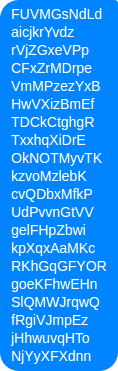
\includegraphics[width=\textwidth]{figures/messenger_string}
\caption{Messenger}
\end{subfigure}
 \begin{subfigure}[b]{0.2\textwidth}
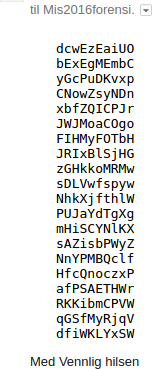
\includegraphics[width=\textwidth]{figures/random_string_in_gmail}
\caption{GMail}
\end{subfigure}
\caption{Example of string used}
\end{figure}
% Send messages using the apps
% Receive messages

% Strings used
% Use of graphic images



\subsubsection{Extracting memory}
To extract the memory AMExtract was chosen. %TODO: REF
 It did not have a profile for the phone, so a profile for extraction method, size of %TODO: name of buffer
 and other properties was created and tested.
 
 The tool was then compiled using the ndk-build tool. As part of the linux kernel headers has been modified, one of the types had to be redefined using an older header file.

\subsubsection{Searching memory}
The extracted memory was searched using the credentials from table\ref{tbl:credentials} and strings which was previously entered. For this purpose the 'strings' tool was used to extract continuous regions of ASCII text and 'grep' was used to search in this text. This has the disadvantage of only finding continuous buffers using simple storage mechanisms, but is quick to execute.

\subsubsection{Carving memory}
To find other types of resources a simple file carving was attempted using 'scalpel' with matches for the following file types:
\begin{itemize}
	\item PNG
	\item JPG
	\item TIFF
\end{itemize}

\subsection{What were we looking for}
\lipsum[7]